\section{結果}
\label{section:experiment__result}

ステッパの学習的効果を評価するため、我々は以下の項目について調査した。

\begin{itemize}
\item ステッパがどれほど使われていたか
\item ステッパをよく使った年と使わなかった年で学生の解答の速さに違いがあったか
\item 学生がステッパについてどう感じたか
\end{itemize}

ステッパがどれほど使われたかについては、 OCaml 実行ログからステッパによる実行とそうでない実行の数を数えた。
解答の速さの差は、チェックシステムに記録されている時刻、
すなわち学生が初めて正解のプログラムをチェックシステムに通した時刻から統計的に分析した。
最後の項目については、学生にアンケートを取った。

% \subsection{The Uses of the Stepper}
\subsection{ステッパの使用状況}
\label{subsection:result__uses}

% We introduced the stepper into Functional Programming in 2016.
我々が授業「関数型言語」にステッパを導入したのは 2016 年度である。
% Although the steppers used in the past had
% almost the same user-interface as the one shown
% in Figure \ref{figure:ocamlfac}, they differ in the following ways:
当時のステッパは図 \ref{figure:ocamlfac} とほとんど同じインタフェースだったが、
以下の点で \ref{section:experiment__stepper} 節で紹介したステッパと異なる。
\begin{description}
% \item[2016] This first version supported function definitions,
% conditionals, records, lists, and recursion.  However, there were
% various operations that were not supported.
% As such, the usability of the stepper was low.
\item[2016年度] 最初の OCaml ステッパは
関数定義、条件分岐、レコード、リスト、再帰のような
より基本的な式しか実行できず、使いにくかった。
% Moreover, when the instructor introduced the stepper to students, he
% only mildly encouraged to use it.
また、教員がステッパを学生に紹介する際に、ステッパの使用を強くは奨励しなかった。
% Although we do not know how much the stepper was used in 2016 since we
% did not log the execution of stepper, we expect it was used
% only rarely in the first few weeks of the course.
2016 年度はステッパによるプログラム実行のログを採取していなかったため
ステッパがどれくらい利用されていたのかは不明であるが、
最初の数週にわずかに利用されたのみだと我々は考えている。
% \item[2017] Based on the lessons from the previous year, the second
% version supported most operations used in the first six weeks.
\item[2017年度] 6 週目までに学習する構文要素のほとんどに対応したステッパを利用した。
% The instructor introduced the stepper up front at the first class and
% showed how to use the stepper with various examples in the subsequent
% classes.
教員は最初の授業で事前にステッパを紹介し、
その後の授業でも様々な例でステッパを利用して見せた。
% \item[2018] The third version supported almost all the constructs
% needed for the course, including modules, exception handling,
% sequential execution, printing, references, and arrays.
\item[2018年度] \ref{section:experiment__stepper} 節で紹介した、
モジュール、例外処理、逐次実行、配列などを実行できるステッパを利用した。
これは授業範囲のほとんどの構文要素を含んでいる。
% It also supported skipping of function application.
また関数適用のスキップ機能も追加した。
% The instructor introduced the stepper as though the stepper was the
% only way to execute OCaml programs, encouraging the uses of the
% stepper.
教員は、まるでステッパでしかプログラムが実行できないかのように学生に紹介することで、
学生にステッパの利用を促した。
% (Students gradually realized that they could execute a program in the
% interpreter in a few weeks.)
(数週の間に学生は普通のインタプリタで実行ができることにだんだん気付いていった。)
\end{description}

\begin{figure}
  \begin{center}
    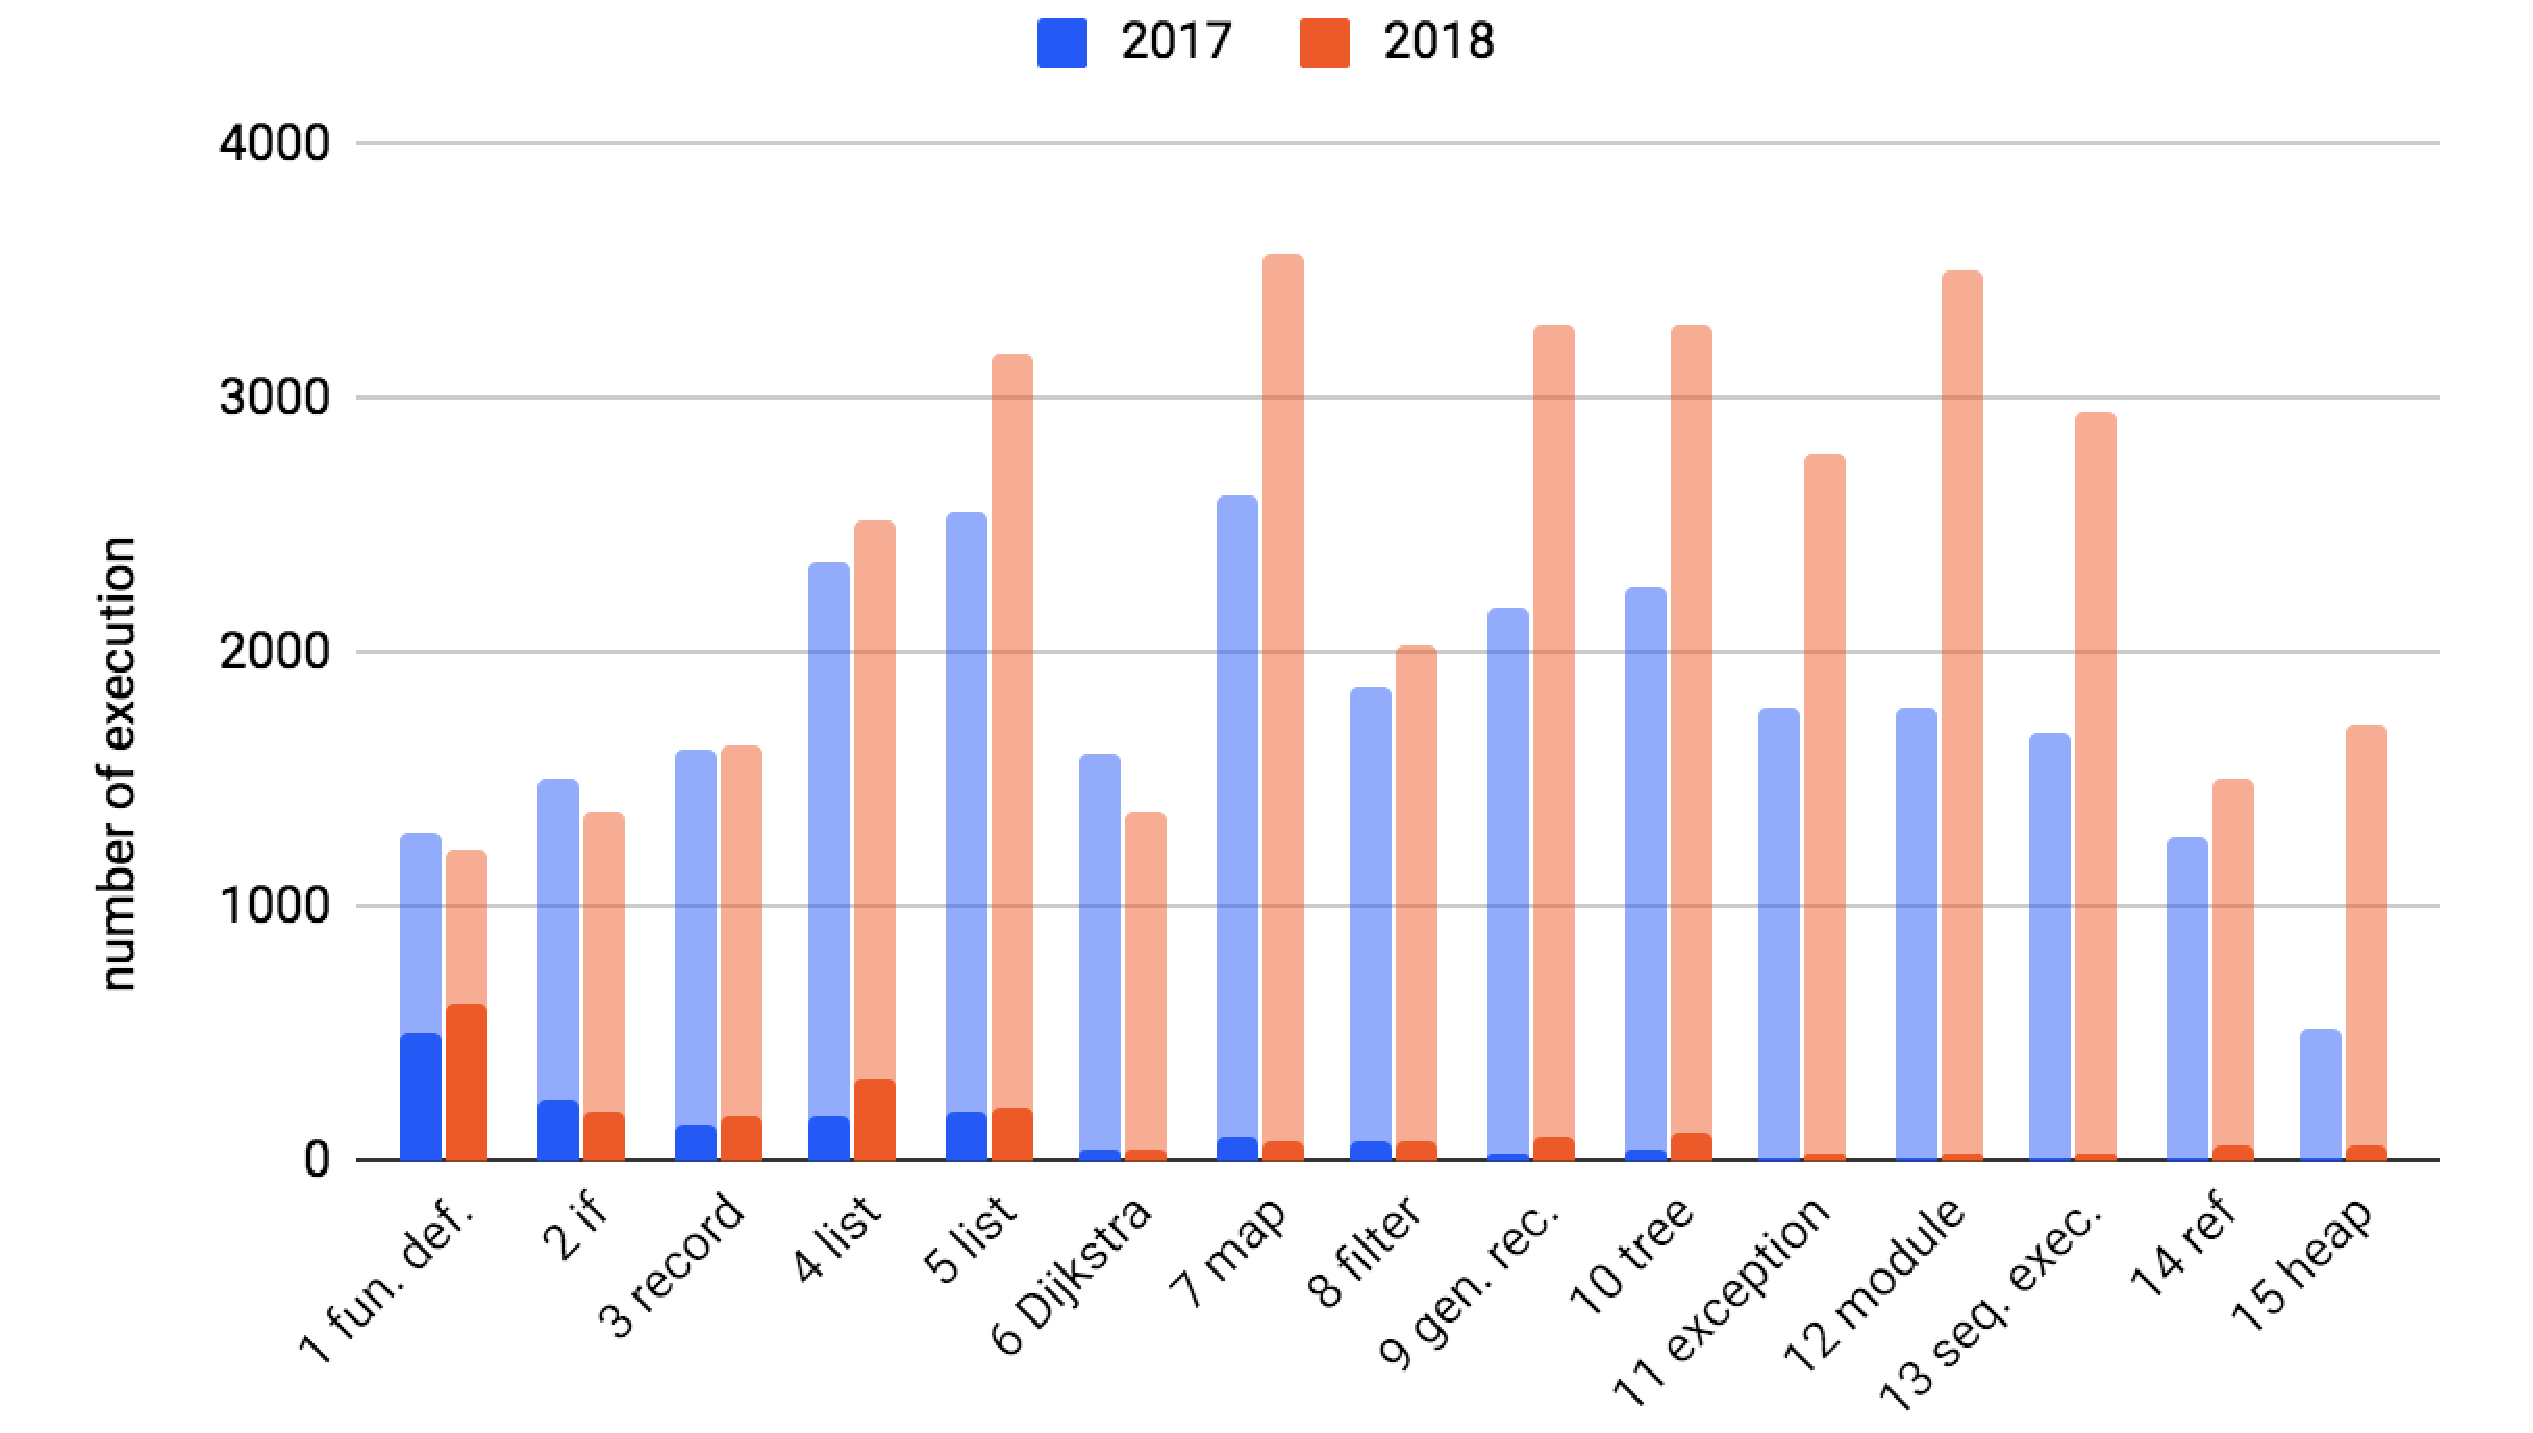
\includegraphics[width=15cm]{6/table1a.eps}
    % \caption{Frequency of standard execution (light-colored) and
    % step execution (dark-colored) in each week in 2017 and 2018.
    % The stepper was not used at all toward the end of the course in 2017,
    % but it was used in some degree in 2018.}
    \caption[ステッパが使用された回数]{
        2017年度と2018年度の各週の、通常の実行 (薄い色) とステップ実行 (濃い色) の回数。
        2017年度は終盤では全く使われなくなったが、2018年度にはある程度使われ続けている。
    }
    \label{figure:allExecution}
  \end{center}
\end{figure}

\begin{figure}[!t]
  \begin{center}
    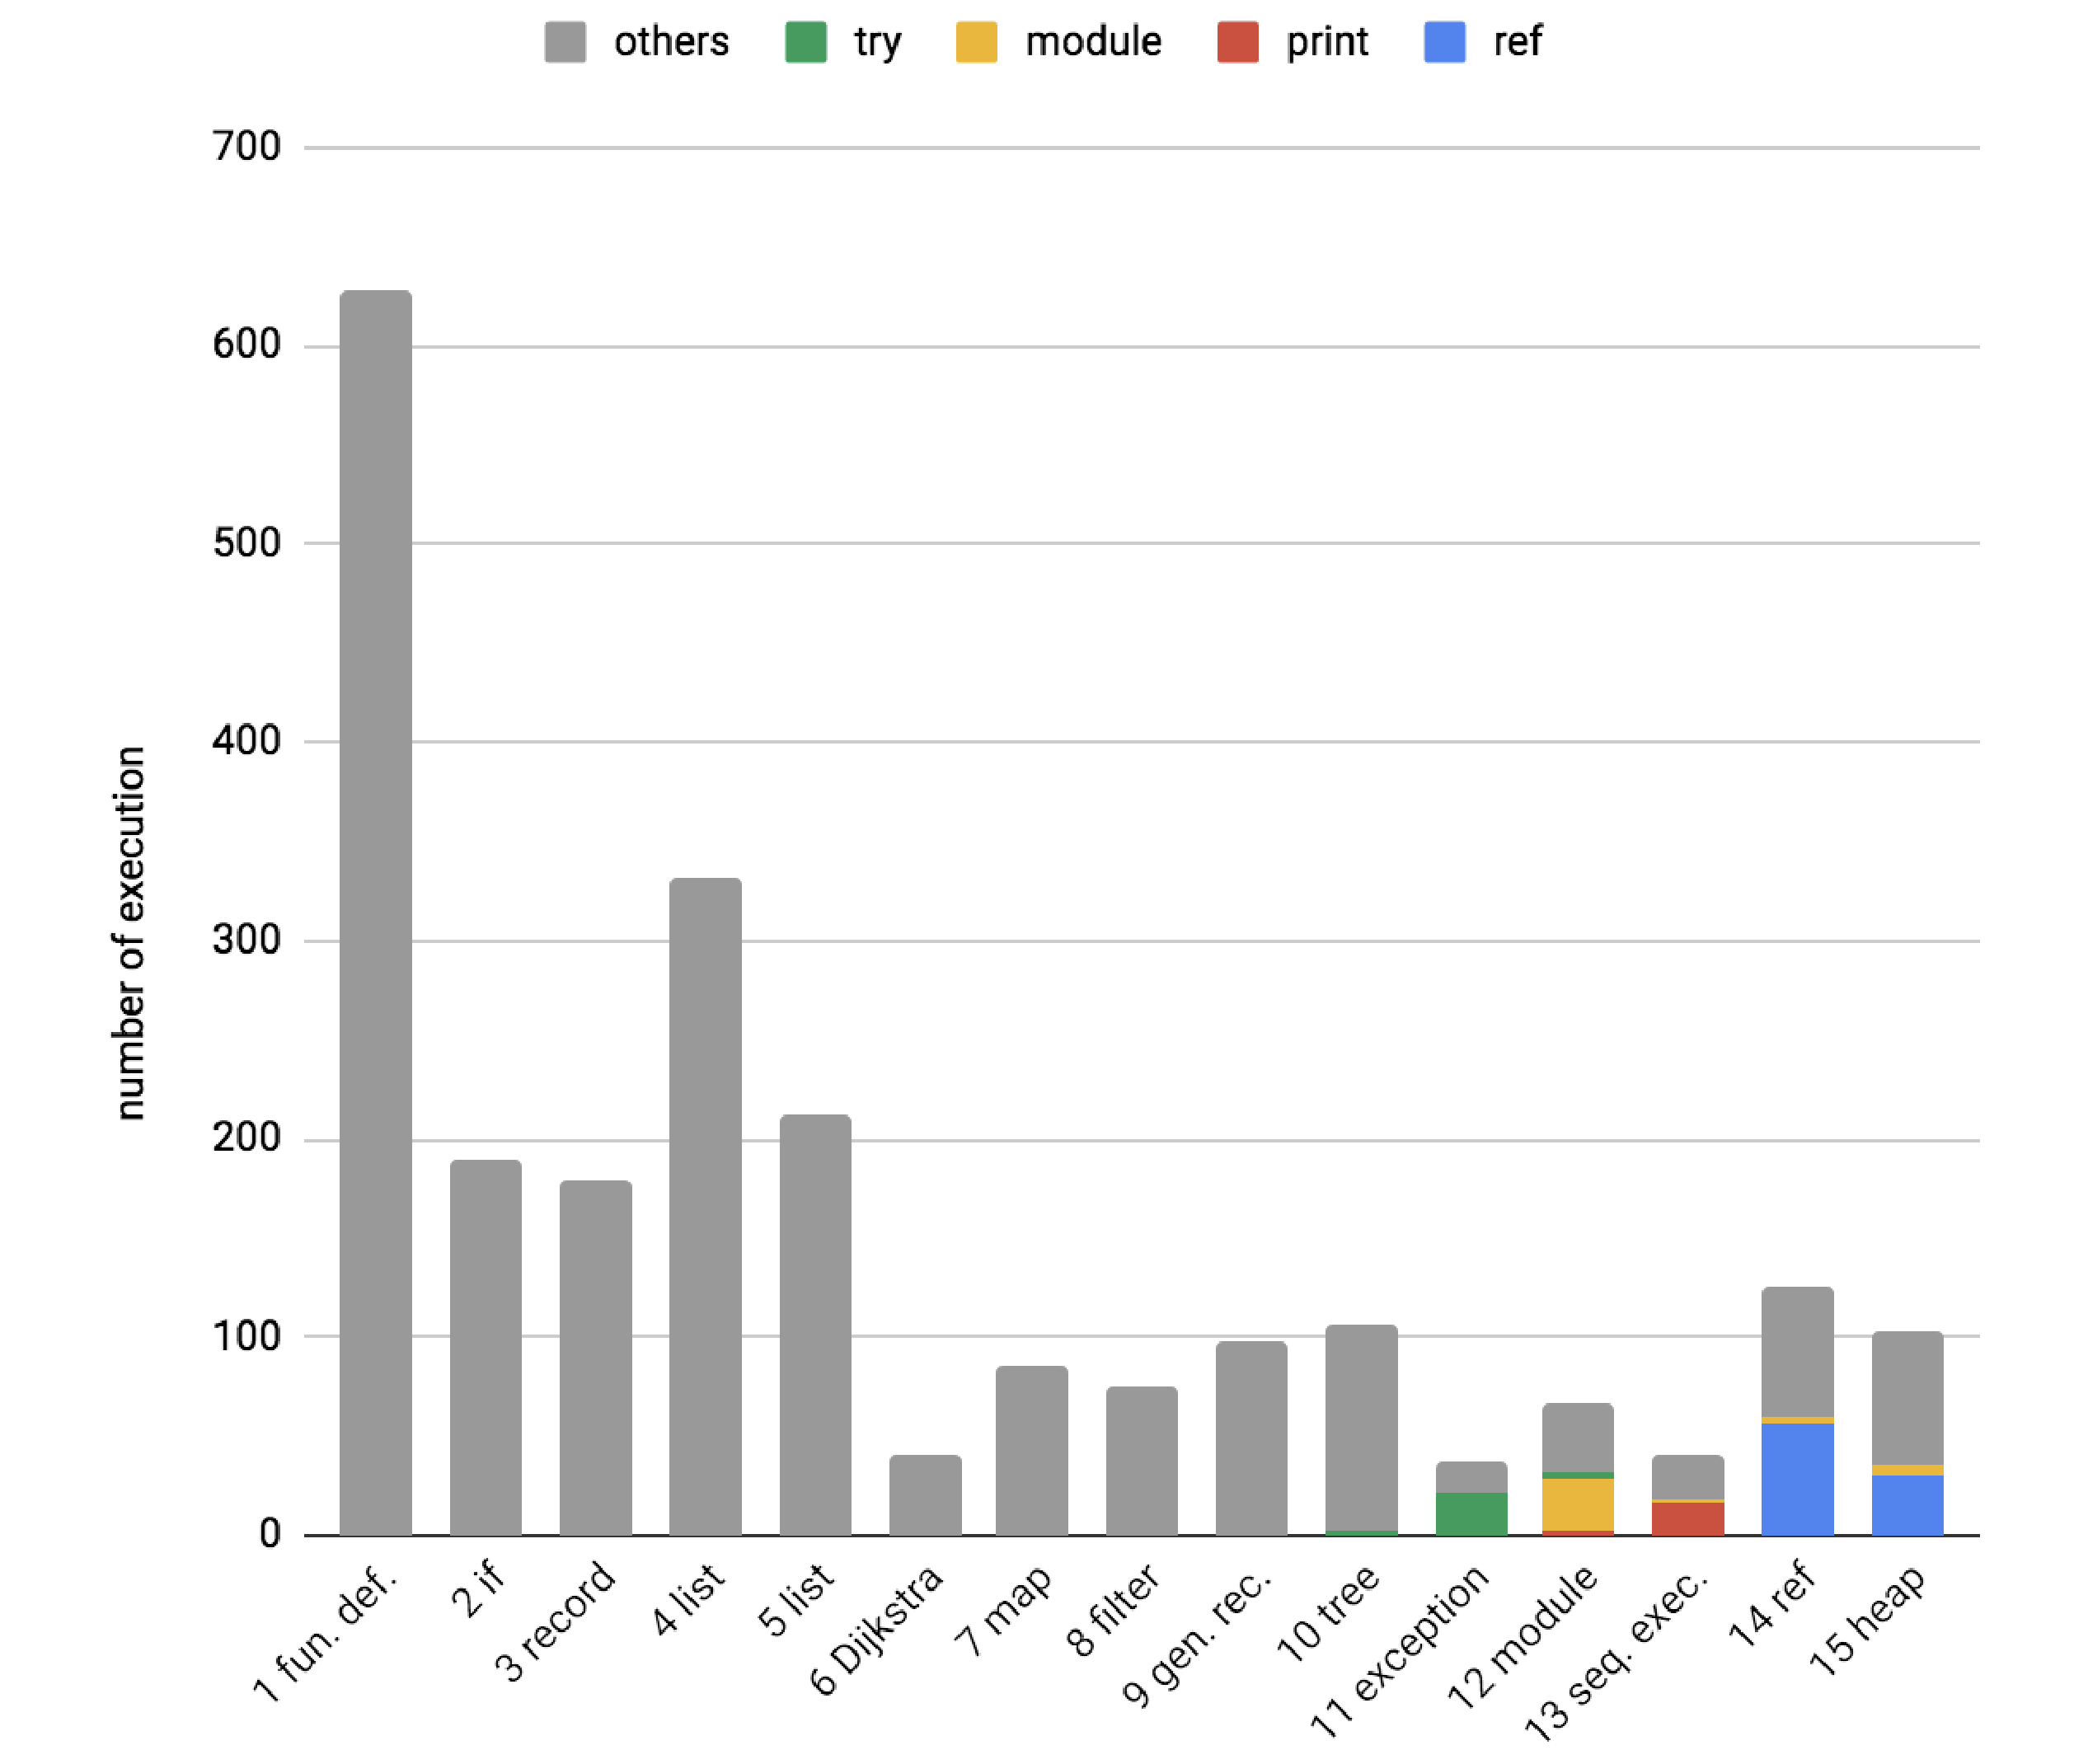
\includegraphics[width=15cm]{6/table1b.eps}
    % \caption{Number of times the stepper was used to evaluate
    % a program with ``try'', ``module'', ``print'' or ``ref'' in 2018.}
    \caption[ステッパの実行のうち各構文を含むプログラムの実行の回数]{
        try、module、print、ref を含むプログラムのステッパによる実行の回数
    }
    \label{figure:stepExecution}
  \end{center}
\end{figure}

% Figure \ref{figure:allExecution} shows
% how many times students used the stepper
% among all the executions including the ones that ended up in an error.
図 \ref{figure:allExecution} は、
全受講生の全実行 (エラー終了した実行を含む) のうち何回がステッパでの実行だったかを示すグラフである。
% In both 2017 and 2018, the stepper was used quite often until week 5.
2017 年度と 2018 年度の両方で、5 週目まではステッパが頻繁に利用されている。
% This is partly because
% we encouraged students to use the stepper when they had
% trouble finding bugs and understanding recursion.
この一因は、バグの発見や再帰の理解のためにステッパを使うように
教員やティーチングアシスタントが学生に勧めたことである。
% After week 5, the number decreases, because students started using an
% interpreter, too, as programs became larger.
6週目以降は、学生がインタプリタに気付き始めたことと
実行するプログラムが大きくなったことにより使用回数が減少した。

% In 2017, the number of stepper uses decreases toward the end of the
% course.
2017 年度には、ステッパの使用回数は最後の授業に近づくにつれて減少している。
% In contrast, in 2018, certain number of stepper uses is observed,
% thanks to the support of exception handling, modules, and references.
それに対して 2018 年度は、例外処理、モジュール、逐次実行、書き換え可能な変数に対応したので、
ある程度の回数の使用が見られる。
% Figure \ref{figure:stepExecution} shows the number of execution of
% programs using these features during step-execution in 2018. % 足した execution を単数にした
図 \ref{figure:stepExecution} は、2018 年度のステップ実行のうち
この年に新しく対応した構文を利用したプログラムの実行の回数のグラフである。
% From the figure, we can see that there is a demand for step
% execution of advanced constructs such as exception handling and
% modules.
どの構文もいくらかステップ実行されており、
例外処理やモジュールのような高度な構文のステップ実行の需要があることが分かる。

% The exact numbers of execution are available in Table \ref{TableUsage} in the Appendix.
図 \ref{figure:allExecution} と図 \ref{figure:stepExecution}
のグラフの正確な数値は付録の表 \ref{TableUsage} に掲載する。

% \subsection{Effects of Stepper}
\subsection{ステッパの効果}
\label{subsection:result__effects}

% It is not easy to see the effect of a tool like a stepper on
% the learning of students.
ステッパのようなツールの教育効果を測ることは簡単ではない。
% In the case of improving error messages of a compiler, for example,
% one can classify various errors and see how many of them are covered
% by the improved error messages objectively.
例えばコンパイラのエラーメッセージ改善の評価ならば、
エラーを分類して改善されたエラーメッセージがそのうちどれほどに対応しているかを見ることができるだろう。
% For the stepper, it is unclear how to show such numeric data.
ステッパにおいては、そういった定量的なデータをどのように示せばよいかが不明瞭である。

\begin{figure}
  \begin{center}
    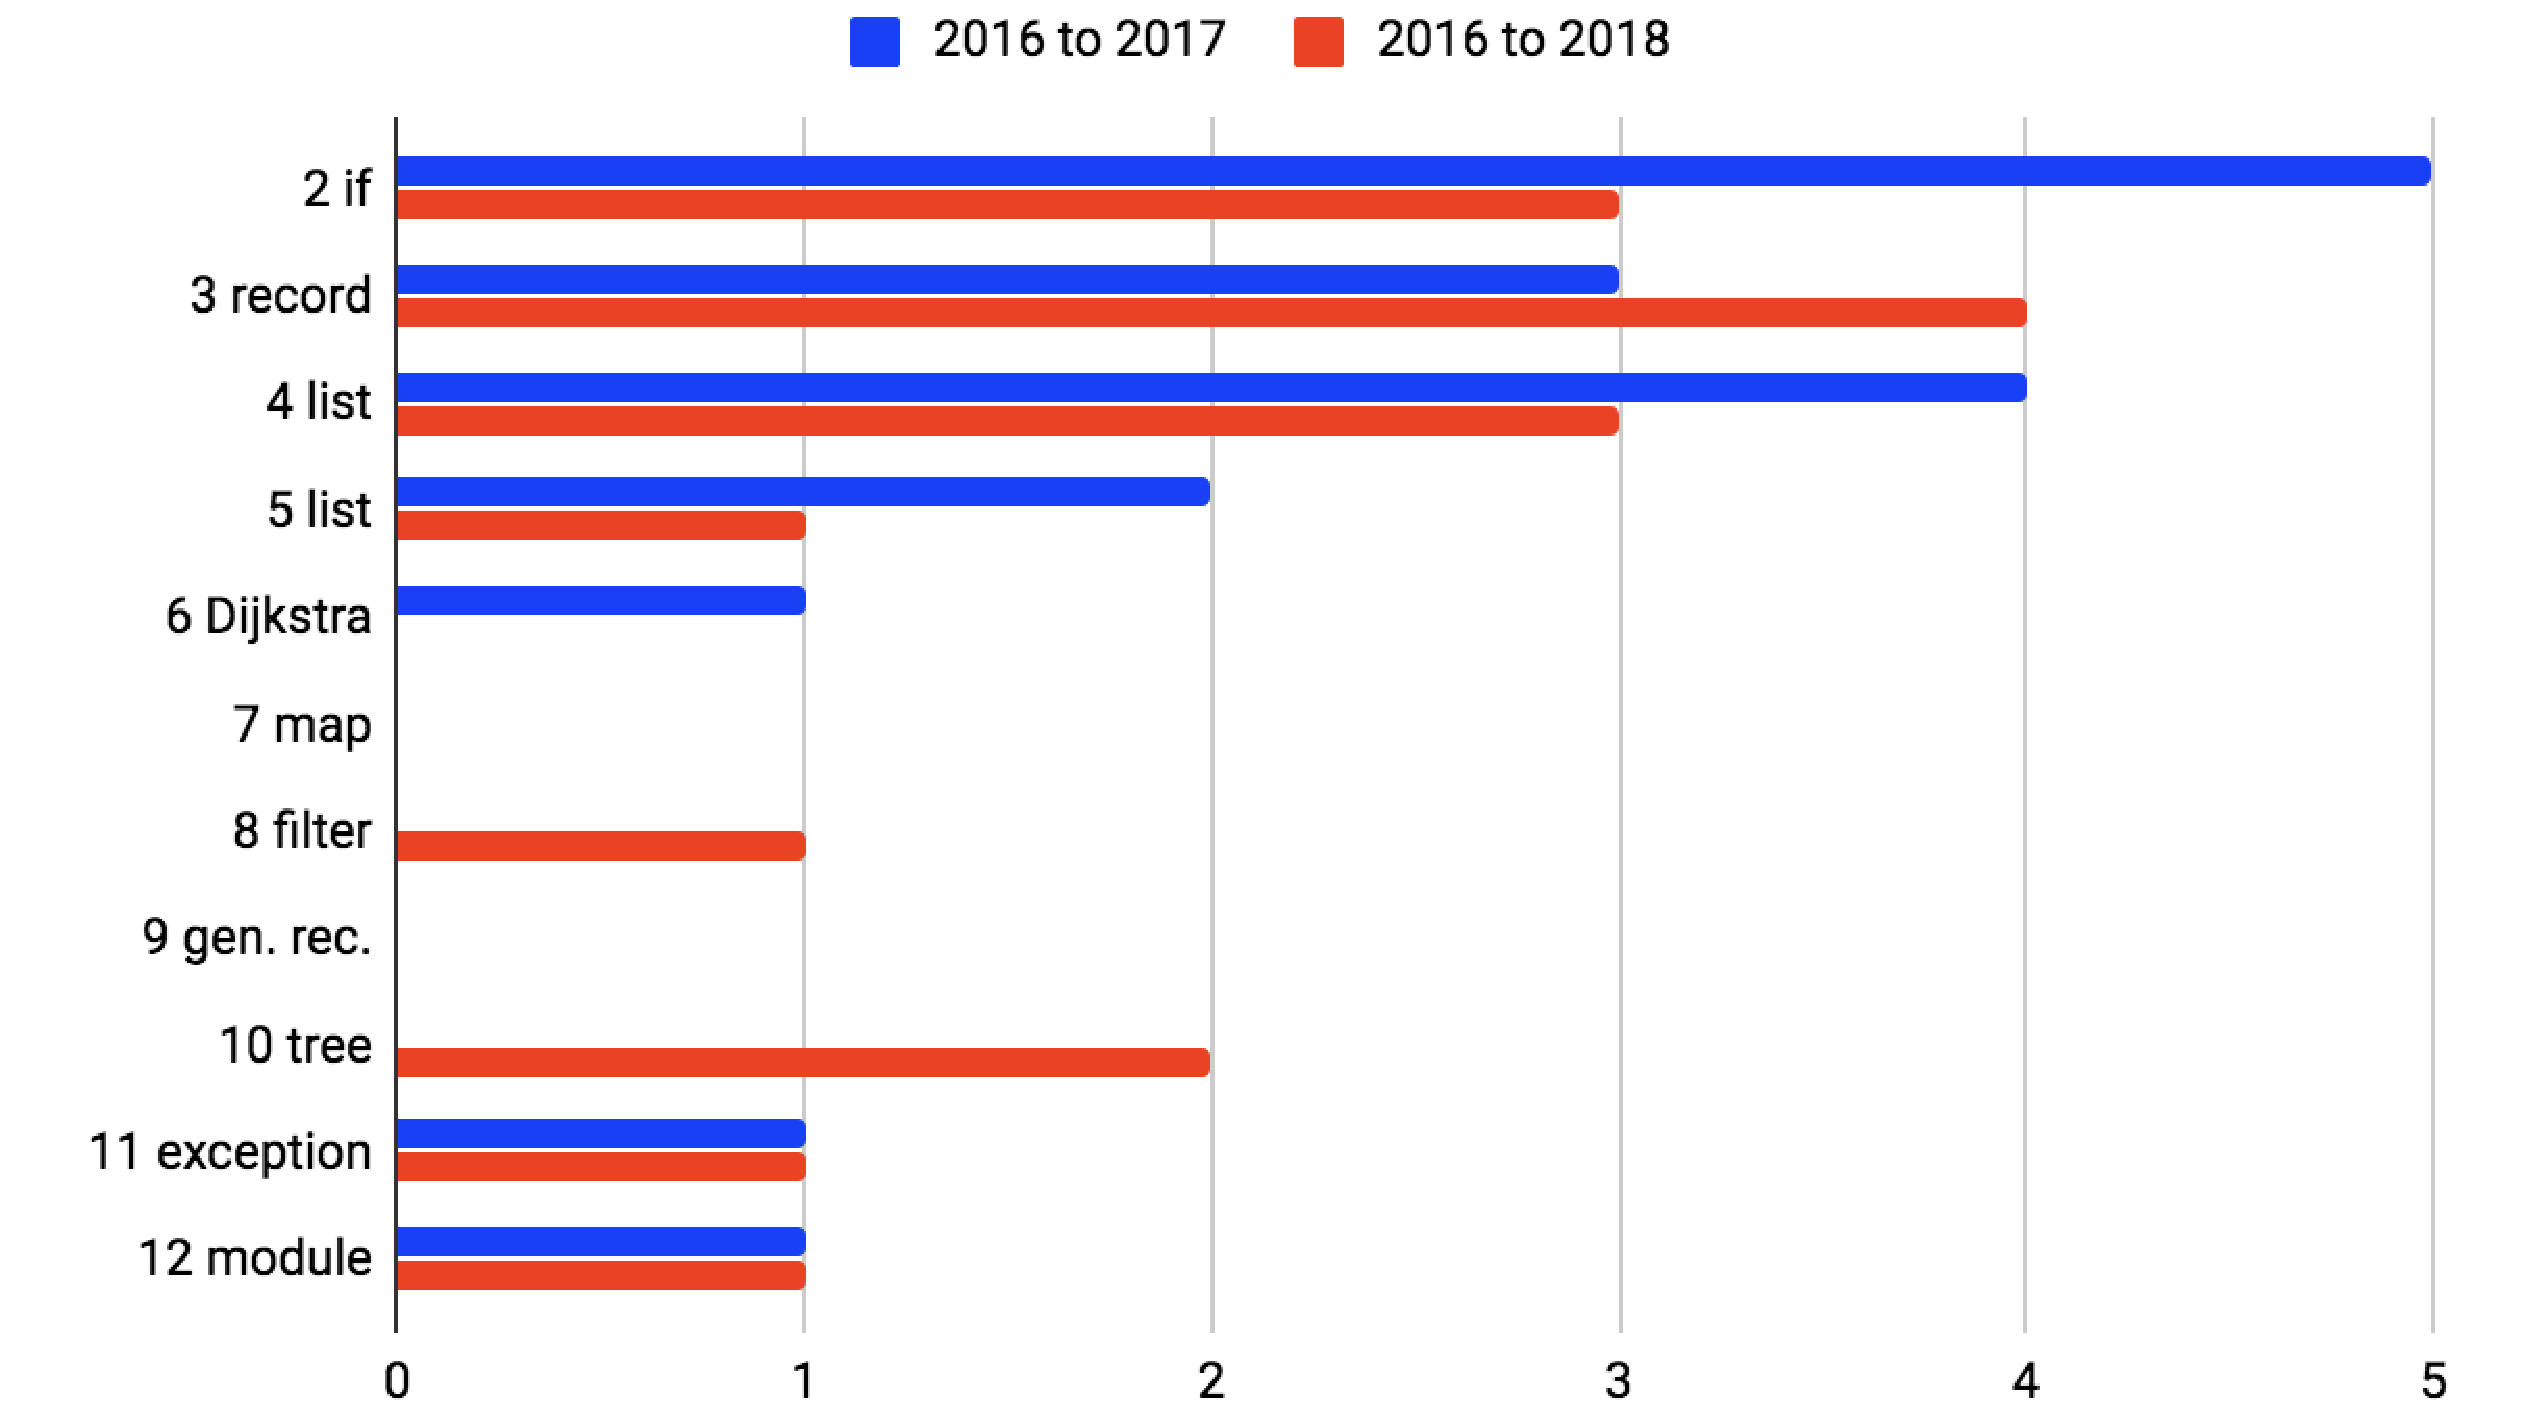
\includegraphics[width=15cm]{6/table2.eps}
    % \caption{Number of questions where students arrived
    % at a correct answer significantly faster in 2017 and 2018 than 2016.}
    \caption[学生が正答するまでの時間の比較]{
        2017年度と2018年度に、学生が2016年度より有意に早く正答を提出した問題の数
    }
    \label{figure:p}
  \end{center}
\end{figure}

% As an attempt to measure the effect of the stepper, we examined how
% long students took to submit correct solutions to the check system.
ステッパの効果を測定するための試みとして、
我々は学生がチェックシステムに正しい解答を提出するまでにかかった時間を調査した。
% Among all the submitted correct solutions, we gathered the (wall-clock) times of
% submissions recorded in the check system that are within 100 minutes
% from the beginning of the class and compared the average times among
% 2016, 2017, and 2018.
全ての問題のチェックシステムに記録されている「正答が初めて提出された時刻」の中から
授業開始から100分以内の時刻を収集し、2016年、2017年、2018年の間で比較した。

% Figure \ref{figure:p} shows the number of questions
% for which students submitted a correct answer
% within significantly shorter time in 2017 and 2018 compared to 2016.
図 \ref{figure:p} は
2017 年度と 2018 年度それぞれの、2016 年度よりも
学生が有意に短い時間で正解を提出した問題の数を示している。
% The data are based on one-sided t-testing with p-value $< 0.05$;
% we refer the reader to Table \ref{TableTTest} of the appendix for details.
このデータは p $< 0.05$ の片側 t 検定に基づいており、
詳しい数値は付録の表 \ref{TableTTest} にある。
% Note that we did not include week 1
% because we had a special pre-test in the first lecture in 2018.
ただし、2018 年度のみ初回の授業に特別なテストを行ったので、
第 1 週はこの調査の対象から外した。

% From the figure, we can see improvement of submission times
% after the (real) introduction of the stepper, especially in earlier problems.
図から、実質的なステッパの導入の後、提出までの時間が改善されていることが分かる。
序盤の問題で特に改善が見られる。
% However, there is an exception: for one problem in the 6th week,
% correct submissions come significantly later in 2018 than in 2016.
しかし 1 つ例外があり、第 6 週の 1 つの問題のみ、
2018 年度の正解提出が有意に 2016 年度よりも遅かった。
% The problem simply asks students
% to write a recursive function that adds 1 to each
% element of a given list.
該当する問題は、リストを受け取ったらそのリストの全要素に 1 を足したリストを返す
再帰関数を書くという単純な問題である。
% We do not know why it took so long in 2018.
この問題の正答が 2018 年度に遅くなった理由は分からない。
% The result of t-testing all the problems together is
% t(1778) = 2.819 (p=0.002) in 2017 and t(2111) = 2.592 (p=0.005) in 2018.
全問題の正答時間をまとめて t 検定した結果は、2017 年度が t(1778) = 2.819 (p=0.002)、
2018 年度が t(2111) = 2.592 (p=0.005) だった。

% We also compared the average times between 2017 and 2018.
2017 年度と 2018 年度の平均時間も比較した。
% For earlier weeks (up to week 5), submissions in 2017 were
% significantly earlier, while for later weeks,
% there were no significant difference
% (except for two problems where the average
% times for 2018 were earlier).
第 5 週までの早い週には 2017 年度の方が有意に早く、
それより後は 2 問のみ 2018 年度の方が早く、あとは有意差は見られなかった。
% Putting all the problems together, the two were not significantly
% different with t(1953)=0.455 (p=0.324).
こちらも全問題の時間をまとめて t 検定すると、t(1953)=0.455 (p=0.324) となり、
有意な差はなかった。

% \paragraph{Threats to validity.}
\paragraph{有効性に対する脅威}
% It is possible that the results of our experiment were affected
% by the enrolled students in each year (there was no over-lapping).
この調査の結果は、各年の学生の影響を受けた可能性がある (同じ学生が 2 度以上履修したことはない)。
% 実験の結果は、毎年入学した学生の影響を受けた可能性があります(重複はありませんでした)。
% In all the three years, 
% the instructor started the class with some introductory comments that
% vary in length.
また、3 年間を通して
毎回の授業時間の最初に教員が前回の課題や今回の内容などについて話す時間をとっており、
その長さは毎回同じではなかった。
% Although the instructor made similar comments in each year, they were
% not exactly the same, which could have affected.
毎年ほとんど同じようなコメントをしてはいるが完全に同じではないので、結果に影響した可能性がある。

% \subsection{Students' Evaluation}
\subsection{学生による評価}
\label{subsection:result__students}

\begin{table}
  \begin{center}
  \begin{tabular}{|l|c|r|}
    \hline
    % & score & \# of students \\ \hline
    & 点数 & 人数 \\ \hline
    % Using the stepper, I could almost always understand & & \\
    % the behavior of programs or the cause of errors. & 4 & 3 \\ \hline
    % Using the stepper, I could often solve problems at hand. & 3 & 8\\ \hline
    % Using the stepper, I could sometimes solve problems at hand. & 2 & 25\\ \hline
    % I could rarely find new things using the stepper. & 1 & 2\\ \hline
    % The stepper was useless.  I did not use the stepper. & 0 & 0\\ \hline
    ステッパを使えばほぼ必ずプログラムの動きや間違いの原因が分かった & 4 & 3\\ \hline
    ステッパを使って問題を解決できることが多くあった & 3 & 8\\ \hline
    たまにステッパを使って問題を解決できることがあった & 2 & 25\\ \hline
    ステッパを使うことで新たに何かが分かることはほとんど無かった & 1 & 2\\ \hline
    全く役に立たなかった、または使わなかった & 0 & 0\\ \hline
%   4 & ステッパを使えばほぼ必ずプログラムの動きや間違いの原因が分かった & 3\\ \hline
%   3 & ステッパを使って問題を解決できることが多くあった & 8\\ \hline
%   2 & たまにステッパを使って問題を解決できることがあった & 25\\ \hline
%   1 & ステッパを使うことで新たに何かが分かることはほとんど無かった & 2\\ \hline
%   0 & 全く役に立たなかった、または使わなかった & 0\\ \hline
  \end{tabular}
  \end{center}
%   \caption{Students' scoring of the stepper in 2018.
%   38 students out of 42 answered.
%   The average is 2.3.}
\caption[学生による点数評価]{2018 年度の学生による点数評価。42 人中 38 人が回答。平均は 2.3 だった。}
% 平均 2.3158、38 / 42 人が回答
  \label{TableScore}
\end{table}

% At the end of the semester of 2018, we asked the students to share
% their thoughts on the stepper.
2018 年度前期の最後に、学生にステッパについてのアンケートを実施した。
% We received responses from 38 out of 42 students.
42 人の受講者のうち 38 人が回答した。
% We first asked whether the stepper was useful on the 0 to 4 point scale.
その中で、ステッパがどれくらい便利だったかを 0 から 4 点で評価してもらった。
% The results, which we present in Table \ref{TableScore}, suggest
% that the stepper is not a silver bullet that is useful
% for all the time.
結果を表 \ref{TableScore} に示す。
この表からはステッパはいつでも役立つ万能なツールではないことが分かる。
% However, most students could solve the problems at hand sometimes
% using the stepper.
しかし、多くの学生がステッパを使って時々問題を解決することができている。
% We are encouraged to see some students choose ``the stepper was almost always useful''.
「ステッパを使えばほぼ必ずプログラムの動きや間違いの原因が分かった」を選んだ学生もいた。

% We next asked students to write when the stepper was useful (if any),
% such as when they found their misunderstanding, or when they could
% deepen their understanding.
他の質問で、
プログラムの間違いの発見や理解のためにステッパを活用できた場面を (あれば) 答えてもらった。
% We summarize the answers in two categories.
その答えを 2 つに分類して紹介する。

% \paragraph{Understanding of the behavior of programs.}
\paragraph{プログラムの挙動の理解}
% Seven students answered they could deepen their understanding of
% the behavior of programs.
7 人の学生が、プログラムの挙動についての理解を深めることができたと答えた。
% In particular, five students among them wrote explicitly that the
% stepper helped them figure out how functions consume recursive data.
特にその内 5 人が関数がどのように再帰的なデータを消費するのかを把握するのに役立ったと書いている。
% 特に、そのうち5人の学生は、関数が再帰データをどのように消費するかを把握するのにステッパーが役立つと明示的に書いています。
% We imagine it was particularly instructive to see how a recursive 
% function definition is unfolded in nesting application.
再帰関数定義が展開されて関数適用の入れ子になっていく様子を見ることができることは
再帰の理解の助けになると考えられる。

% Other students answered that they could observe the behavior of
% programs in general.
他の学生は、プログラム全般の動きを観察できたと答えた。
% They found that arguments of a function are evaluated before the
% function call, and that the elements of a list are evaluated one by one.
その学生たちは、引数が関数呼び出しの前に 1 つずつ実行されることを発見した。
% Among them, one student observed the right-to-left execution
% employed in OCaml.
1 人は OCaml プログラムが right-to-left で実行されていることに気付いた。
% Previously, such subtle behavior was taught only in passing without
% much emphasis.
以前は、このような細かい動作について特に強調せず授業を進めていた。

% \paragraph{Debugging.}
\paragraph{デバッグ}
% Many students found the stepper useful for debugging.
多くの学生がデバッグにステッパを利用できたと回答した。
% Sixteen students answered they could find what was wrong when their
% program did not pass test cases.
16 人の学生が、テストを通らなかった時にどこが間違っているのかを見つけることができたと回答した。
% By observing each step of execution, they could identify when the
% program behaved differently from their expectation.
実行の各ステップを観察することで、期待と違った振る舞いをする箇所を特定することができたという。
% This is an important step toward debugging in general.
これは一般的なデバッグをする上で重要な過程である。
% Because printing (and side effects) is handled at the end of the
% course, the only debugging method for students had been unit testing:
% they checked whether all the component functions worked as expected.
この授業では出力などの副作用を終盤で学習するので、
学生のデバッグの方法は単体テストで関数全体が正しい値を返すかどうかを見るしかなかった。
% With the stepper, they can simply observe execution of the program and
% see when it goes wrong.
しかしステッパがあれば、
学生は実行中のどこで間違いが起きているのかを単純に観察することができる。

% Three students found the stepper useful to understand why their
% program did not terminate.
% Without printing, it is not easy for students to identify the cause of
% infinite loops.
また、3 人の学生がプログラムが停止しない時にその原因をステッパで突き止めることができた。
出力機能を使わずに無限ループの原因を特定することにもステッパは利用できる。
% Using the stepper, one of the students could not only observe
% the infinite loop, but also see how far her progr went well
% and when it went wrong.
% ここは書かない・・・
